\chapter[Literature review]{Literature review }
\label{Chap:label}	%CREATE YOUR OWN LABEL.
\pagestyle{headings}

This chapter introduces the necessary topics in relation to the project. These topics include, field programmable gate arrays, packet filter firewalls, RISC-V processors, Ethernet MAC, webs servers and network stacks.  








\section{Packet Filter Firewall}

Usually, the first line of defence against bad actors, firewalls play a vital component in computer networks and as such can become vastly complex. 
In essence, the job of a firewall is to isolate and restrict access to an internal network from an external one to increase security \cite{BuildingInternetFirewalls}.

There are several types of firewalls such as packet filters (PF), stateful packet firewalls and application firewalls \cite{FirewallsBook}. 
Traditional PFs are considered as stateless and filter exclusively on the fields in the network and transport layer headers \cite{FirewallsBook}. More information on the different layers in a network can be found in section \ref{sec:computer_networks}. Such fields include IP addresses, port numbers and protocol type.

Due to this, PFs are inherently simple, efficient and relatively effective in most situations. As a result, they are widely available and can be either implemented in software or in hardware \cite{BuildingInternetFirewalls}. The book, \cite{BuildingInternetFirewalls}, also highlights some inherent flaws with PFs which include not being able to suppress sophisticated attacks and in some cases, can be challenging to properly configure. More advanced firewalls can perform deep packet inspection which explore the contents of the higher layers and factor in previous packets to better evaluate a packets true intention \cite{FirewallsBook}. 

While firewalls such as \textit{iptables} in Linux are software based, hardware acceleration can vastly improve the performance of a packet filter. As mentioned in section \ref{subsection:fpga}, hardware acceleration allows for parallelised algorithms to be executed independently of a central processing unit (CPU). Wicaksana and Sasongko, \cite{FastRecongifFPGAFirewall}, proposed a packet classification engine as shown in figure \ref{fig:fast-fpga-classifier}. To obtain a fast yet reconfigurable and scalable packet classifier, the authors of \cite{FastRecongifFPGAFirewall} used a hierarchical tree-based algorithm that inspects the multidimensional fields of the IP header through the use of parallel decision trees.

Essentially, the architecture in figure \ref{fig:fast-fpga-classifier} employs memory to store the ruleset and uses a multiplexer and a comparator to evaluate each of the fields in the header. As a safegaurd, the authors opted for a \textit{default-deny} ruleset to prevent any unwanted traffic. One inherent downside to this design is that it requires additional clock cycles for each rule that gets added to the ruleset. 


\begin{figure}[h]
    \centering
    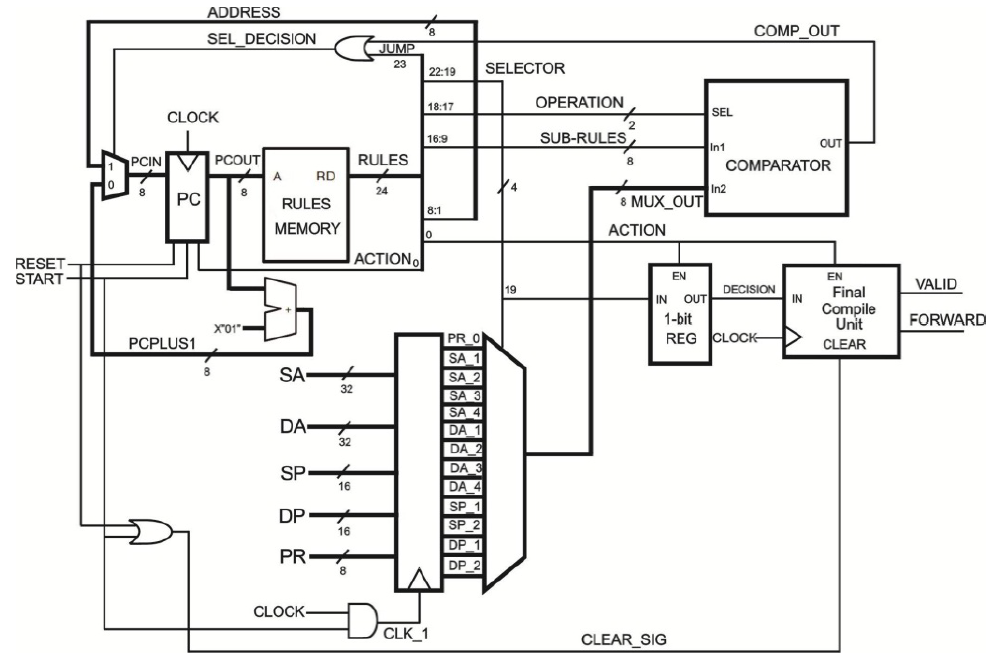
\includegraphics[width=0.8\textwidth]{Images/packetFilterHardware.png}
    \caption[Packet classifier]{Packet classifier \cite{FastRecongifFPGAFirewall}}
    \label{fig:fast-fpga-classifier}
\end{figure}


Wasti \cite{Wasti2001HardwareAP} presents several other classification algorithms for both hardware and software packet filters. \textit{'Sequential matching'} provides the most trivial solution as it matches each rule to the incoming packet. While simple, this design has scalability issues as more rules get added. Another method proposed in \cite{Wasti2001HardwareAP} is by using a \textit{'Grid of tries'} which uses tries (a type of tree datastructure) to help pattern match the packets, but fails to extend to multiple fields. 
Hardware algorithms using \textit{Ternary CAMs} (stores words with 3-valued-digits - namely '0', '1' and '*') and \textit{Bit-parallelism} were also discussed. Both of these exploited the parallelised nature of hardware design. One limiting factor with the classification methods cited in \cite{Wasti2001HardwareAP} is their configurability and expandability. 








\section{Field Programmable Gate Arrays}
\label{subsection:fpga}	
First introduced by Xilinx in 1984, field programmable gate arrays (FPGAs) allowed for large custom logic designs to be recognised without the need for 
expensive application specific integrated circuits (ASICs). More importantly, FPGAs did not suffer from the same scalability issues that
programmable array logic (PAL) encountered and has allowed for larger and more complex designs \cite{30YearsOfFPGA}. 

A large advantage to custom logic is the ability to create highly parallelised designs with lower latencies and higher throughput than software-based serialised algorithms. This comes down to 
having a great degree of freedom when it comes to designing the architecture and ability to optimise for specific tasks.
As such, FPGAs have became ubiquitous in both digital signal processing and for accelerating an assortment of heterogeneous computing architectures and processes including networking \cite{FPGAComputing}.
More specifically, system on chip (SoC) design with custom hardware acceleration modules is an active area research. As \cite{FPGAComputing} points out, there is a focus towards using both hardware and software in \textit{edge devices}\footnote[1]{\textit{Edge devices} are a result of the edge computing paradigm which moves computation closer to the source \cite{EdgeComputing}} due to growing numbers of IoT devices.


Several papers, \cite{LwIPFPGAFirewall} \cite{IPFPGAFirewall2000} \cite{packetFilteringFPGA}, have proposed a range of related FPGA based firewalls that have different properties and focus on different optimisations. The key benefit to these firewalls is their high performance - namely, low latency, and high throughput. 
Article \cite{LwIPFPGAFirewall} proposed an Ethernet firewall using LwIP (A TCP/IP stack) with five-tuple binding (the five filtered parameters in packet filters) 
to achieve a throughput of 950Mbps with a latency of 61.266us. A conference proceeding in 2000 \cite{IPFPGAFirewall2000} used a comparator unit to check the fields of the IP headers obtained a filtering rate of 500,000 packets per second. 


The enabling concept behind the above FPGA based firewalls is SoC design which involves integrating multiple components into a single package, or in this case a 
single FPGA. Often these will include small softcore microprocessors and some custom hardware such as Ethernet controllers or packet filtering hardware like the proposed designs in \cite{LwIPFPGAFirewall}.
Having a microprocessor in the FPGA design can significantly reduce the complexity of the design and allows for quick and easy development in software instead of hardware \cite{SoftcoreBasedEmbeddedSystems}. In FPGA design, softcore processors are generally highly configurable and can be modelled in a hardware description language (HDL) which can then be synthesised onto ASICs or FPGAs hardware \cite{SoftcoreBasedEmbeddedSystems}. There are several softcore processor architectures available for FPGA designs including ARM Cortex, Nios II, MicroBlaze, and RISC-V. 
 
While recently the royalty free RISC-V based cores have been popular amongst many SoC designs, other older processors are still common in the literature. The two big FPGA vendors, Xilinx (now AMD) and Altera (now Intel) have their own RISC based softcores. As an example, Janik et al. \cite{LwIPMicroblaze} used Xilinx's MicroBlaze processor as a media converter between optical (SFP interface) and copper (Ethernet) networks. Likewise, Altera's Nios II can be found in a variety of research papers including an embedded web server which significantly simplified the design \cite{NiosIIWebserver}. 

 







\section{RISC-V processor}
There are four major processor architecture families, namely AMD64, x86, ARM and RISC-V. The two former instruction set architectures (ISA) 
are a part of the complex instructions sets (CISC) and are found in the majority of computers such as laptops and servers. ARM and RISC-V have a reduced instruction set compared to the CISC family and subsequently fall under the RISC family and are ideal for low power microprocessors \cite{RV16Embedded}.

RISC-V is an open and royalty free ISA and as a result, a plethora of softcore based custom implementations have been designed and are available for use in designs\cite{CatalogRISCSoftcore}. 
Consequently, there is an abundance of articles delving into RISC-V from evaluating the ISA \cite{InvestigatingRiscv} to creating multicore architectures
\cite{RiscVMulticore}. A 2019 paper, \cite{CatalogRISCSoftcore} evaluated a variety of different RISC-V softcore processors. RISC-V International have 
also published a list\footnote[1]{See: https://github.com/riscv/riscv-isa-manual/blob/master/marchid.md} of different RISC-V implementations 
that have a unique architecture ID. The majority of these are either written in a HDL for either application specific integrated circuits (ASICs) or FPGAs.
The \textit{NEORV32 RISC-V} softcore processor is written purely in vendor-agnostic VHDL and importantly has a considerable amount of documentation. The design is regularly updated by the maintainers with the original creator, Stephan Nolting, emphasising the importance of understandability. 

Being a softcore processor, control is given over which modules are implemented. Some basic features of the \textit{NEORV32 RISC-V} include 
UART, SPI, and GPIO interfaces \cite{neorv32Datasheet}. The datasheet, \cite{neorv32Datasheet}, also mentions that it supports a \textit{'Wishbone b4 classic'} 
external bus interface. A Wishbone B4 (or just 'wishbone') interconnection is designed specifically to connect modular pieces of hardware together on a 
SoC into the memory mapped 32bit address space in the processor \cite{WishboneSpec}. This translates into accessing the hardware as a bunch of regular memory accesses like setting any other registers or values stored in main memory. This approach results in the benefit of not needing to create custom 
instructions for the microprocessor. 







\section{Computer Networks}
\label{sec:computer_networks}
To understand how one might go about creating an Ethernet interface and firewall, it is important to understand how networks operate. The TCP/IP model is a layered model that blueprints the different protocols and standards used in computer networks so that two devices can communicate in a prescriptive way. 
Figure \ref{fig:tcp_ip_model} shows the updated five layers of the TCP/IP model mentioned in \cite{ciscoCCNABook}.


\begin{figure}[H]
    \centering
    \begin{tikzpicture}[layer/.style={rectangle, draw=black, align=center, text width=3cm, minimum height=1cm}]
        \node (application) [layer] {Application};
        \node (transport) [layer, below=0cm of application] {Transport};
        \node (internet) [layer, below=0cm of transport] {Network};
        \node (link) [layer, below=0cm of internet, fill=lightergray] {Data Link};
        \node (physical) [layer, below=0cm of link] {Physical};
    \end{tikzpicture}
    \caption{Updated Layers of the TCP/IP model}
    \label{fig:tcp_ip_model}
\end{figure}

Each layer provides a service to the layer above it and is typically processed and handled by a separate process in either hardware or software. The physical layer is responsible for the transmission and reception of the above layers over a physical medium such as copper, radio frequency or fibre optics. 

The data link layer (layer two, coloured grey) is responsible for the physical addressing of devices on the network and \textit{links} devices together. Ethernet is the most common protocol used in the data link layer and will be discussed in \ref{sec:eth_mac_lit} and throughout the thesis. Other protocols such as Point-to-Point Protocol (PPP) also exist \cite{ciscoCCNABook}.

The network layer (layer three) is responsible for addressing and routing of packets between networks and devices. The services this layer provides is one that is analogous to a regular postal service. The one major protocol used in this layer is Internet Protocol (IP) and it works by comparing known addresses in a routing table to the destination address of the packet \cite{ciscoCCNABook}. RFC791 \cite{rfc791}, defines all the protocol headers and how it operates.

The transport layer (layer four) is responsible for the end-to-end communication between devices and is where the TCP and UDP protocols reside. The application layer (layer five) is what is used for application specific protocols such as HTTP, FTP, and DNS.





\section{Ethernet Media Access Control}
\label{sec:eth_mac_lit}

First introduced in 1983, the IEEE 802.3 standard \cite{IEEE802.3-2012}, more commonly known by the name of 'Ethernet', defines the \textit{'Medium Access Control'} (MAC) protocol amongst other things for two or more devices to communicate over a network at layer two. 

A core function of the Ethernet MAC is to attach the required MAC headers and preamble to the head and tail of the layer 3 payload to create an Ethernet packet. The fields in an Ethernet packet can be seen in figure \ref{fig:ieee-mac-headers}. 

\begin{figure}[h]
    \centering
    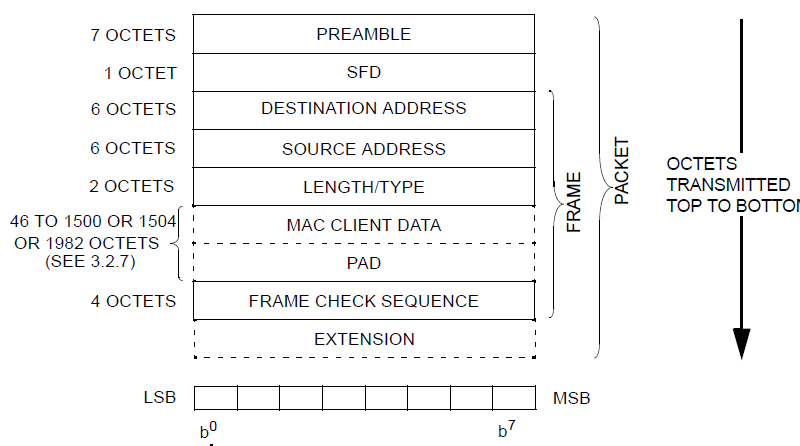
\includegraphics[width=0.65\textwidth]{Images/mac_packet.png}
    \caption[MAC layer headers]{MAC layer headers \cite{IEEE802.3-2012}}
    \label{fig:ieee-mac-headers}
\end{figure}

The preamble and start frame delimiter (SFD) is used to synchronise the physical interface (PHY) and get it ready to send out data and is typically omitted when passing data up to higher layers such as for inspection with tools like Wireshark.

After the packet has been constructed, the data is forwarded to the PHY least significant bit (LSB) first \cite{IEEE802.3-2012}. Typically, a PHY management chip is used to handle the physical layer channel encoding and scrambling amongst other things. 
These PHY chips can often be interfaced with the media independent interfaces such as MII, RMII, GMII and RGMII \cite{OptimisedEthernetMAC}. The Reduced Media Independent Interface (RMII) is one of these standards defined in \cite{IEEE802.3-2012} and consists of a reference clock, 2 bit wide transmit (TX), 2 bit wide receive (RX) lines and a few other supplementary signals like defined in the LAN8720A datasheet, an example RMII PHY \cite{LAN8720ADatasheet}.


The MAC layer itself is usually implemented in hardware as it has several advantages over a software implementation. The core reasons behind this are due to parallelised nature of hardware and that parts of the MAC can operate independently \cite{reducedEtherentMacFPGA} of each other. One key example is the calculation of the Frame Check Sequence (FCS in figure \ref{fig:ieee-mac-headers}). The FCS for Ethernet is a 32bit cyclic redundancy check (CRC) \cite{IEEE802.3-2012}. CRC32 is not unique to Ethernet, but rather can be found in an extensive amount of applications. As such, prior research into parallelised architectures for the calculation have been made by others. Noteably, Mitra and Nayak \cite{ParallelCRC} proposed a low latency parallelised architecture for FPGA design on CRC32. As a result, packets can be assembled faster and offload additional processing burden from the CPU. 


Numerous articles, \cite{OptimisedEthernetMAC} \cite{EthernetAXI} \cite{EthernetRMII}, can be found about implementing Ethernet MACs 
on FPGAs each with a slightly different approach and focusing on different properties. Fundamentally though, as best highlighted in \cite{OptimisedEthernetMAC}, a simple way of implementing a MAC is by employing a finite state machine (FSM) to set the required fields and send out the packet. Another technique found in these articles is to use first-in first-out (FIFO) buffers to cross clock domains as the PHY speed likely won't match the clock frequency of the rest of the system. This is a common technique used in FPGA design as it allows you to have the packet assembly logic at a much higher clock rate than the output RMII reference clock speed \cite{EthernetAXI}. 


The source address field is typically filled in by hardware and is fixed as the MAC address is supposed to be globally unique to prevent address clashes on the same network. The destination address is typically set by software however as the ARP (Address Resolution Protocol) tables are typically stored in software due to them storing a mapping between the layer three IP addresses and the MAC addresses to forward a packet to. 

The Length/Type field has a dual purpose, and it depends on the value. If a value is less than or equal to 1500, then it indicates the size of the packet. While if a value of greater than 1500, then it indicates the type of packet, called EtherType \footnote[1]{See https://en.wikipedia.org/wiki/EtherType for the different types}. Common values are 0x0800 for IPv4 packets and 0x0806 for ARP. Like with the destination address, this is usually populated by software as the type is dependent on the above layers.


In addition to the papers, there are a plethora of intellectual property (IP) blocks for xMII interfaces in HDL 
which have their own benefits and drawbacks. Some freely available HDL modules for Ethernet MACs can be found in both a complete \footnote[2]{See: https://github.com/yol/ethernet\_mac} \footnote[3]{See: https://github.com/alexforencich/verilog-ethernet/} 
\footnote[4]{See: https://opencores.org/projects/ethernet\_tri\_mode} and incomplete state
\footnote[5]{See: https://github.com/pabennett/ethernet\_mac}.








\section{Web servers and network stacks}



Almost all firewalls need to be configured with a ruleset which can be configured in two common ways, using a command line interface (CLI) 
or by a web-based graphical user interface (GUI). Before a web server can be realised, the network stack (Layers 3, and 4) need to be established since a web server operates at the application layer (layer 5). As embedded platforms are resource limited, special precautions need to be taken into consideration when it comes to memory and resource usage \cite{OptimCortexLwIP}.

Article \cite{LwIPFPGAFirewall} investigated using the open source lightweight IP (LwIP) network stack as a mechanism for interfacing with the firewall. 
The LwIP library is a popular lightweight TCP/IP stack which has been investigated in a plethora of research papers and projects \cite{ImprovemntOptimLWIP} 
\cite{OptimCortexLwIP}. Often these papers run LwIP on real time operating systems (RTOS) such as FreeRTOS or Zephyr. These provide an abstraction to the hardware that allows for multitasking and brings other OS-Like features to embedded systems. 

LwIP is not threadsafe and typically suffers from memory issues as found in \cite{OptimCortexLwIP}. However, FreeRTOS's own TCP/IP network stack called \textit{FreeRTOS-Plus-TCP} provides a threadsafe Berkley sockets API and is newer. Consequently, less research can be found apart from existing documentation. These libraries typically implement multiple protocols such as DHCP, DNS, TCP, and UDP \cite{FreeRTOSTCP}.

RFC2616 \cite{rfc2616}, defines the HTTP protocol used by all browsers and web servers and includes the formatting, allowed characters and the different request methods for each packet. HTTP1.1 and HTTP2 use TCP, typically on port 80, to communicate between the client and the server. However, HTTP3 uses the UDP protocol as defined in RFC9114 \cite{rfc9114}. For the remainder of this thesis \textit{'HTTP'} will be used to refer to HTTP1.1.

The HTTP specification, \cite{rfc2616}, defines the protocol as a stateless request-response type where the client first initiates a request to the server and the server responds with a status code and the requested data such as HTML data or images. \textit{GET} and \textit{POST} requests are the most common type and allow data to be retrieved and sent to the server. Since the browser renders the received HTML the data on screen, the webserver only needs to forward the raw HTML data (which can be stored on physical media) to the client.